\section{Owner interface}

When you do the registration as an owner, the application will create
automatically a restaurant with the name equal to your selected username (for
example, a new user named ``User1'' has a default restaurant’s name which is
``User1’s Restaurant'').

Figure~\ref{fig:owneriface} shows the Owner interface.

\begin{figure}[!ht]
	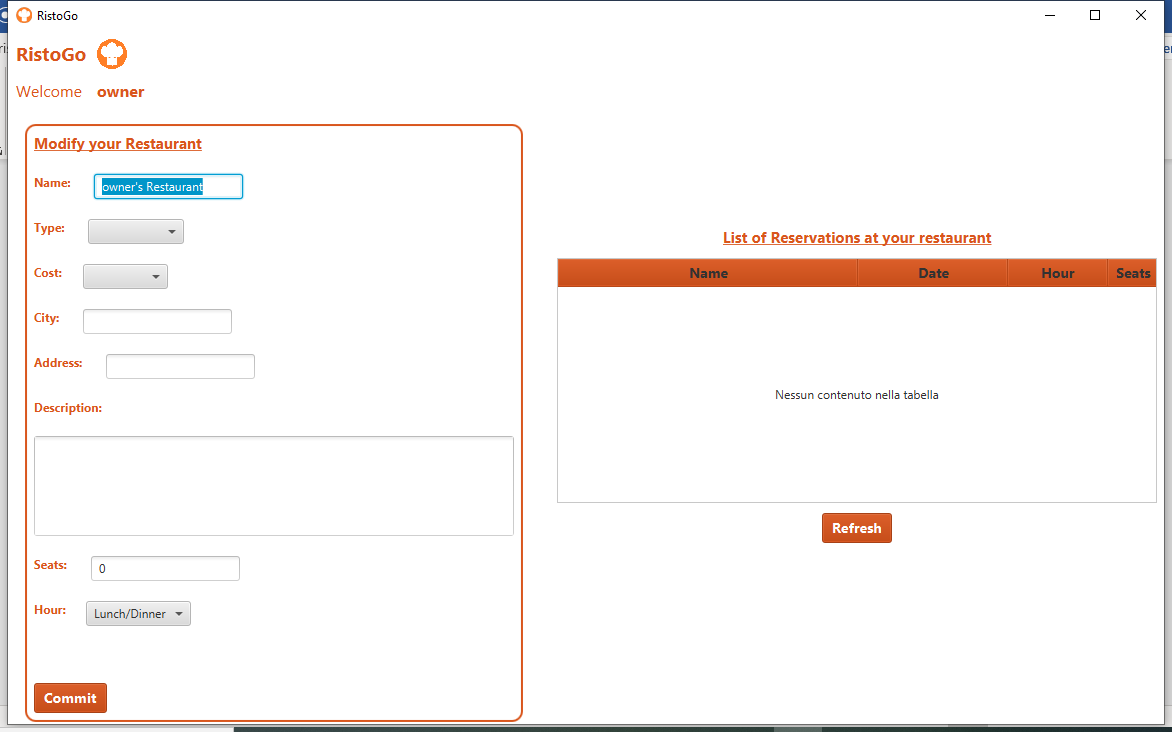
\includegraphics[width=\textwidth]{owneriface}
	\caption{Owner interface.}
	\label{fig:owneriface}
\end{figure}

\subsection{Modify restaurant informations}

After the first login you can change your restaurant’s informations, filling the
form on the section ``Modify your restaurant''. Then click on the button
``Commit'' (Figure~\ref{fig:editrestaurant}).

\begin{figure}[!ht]
	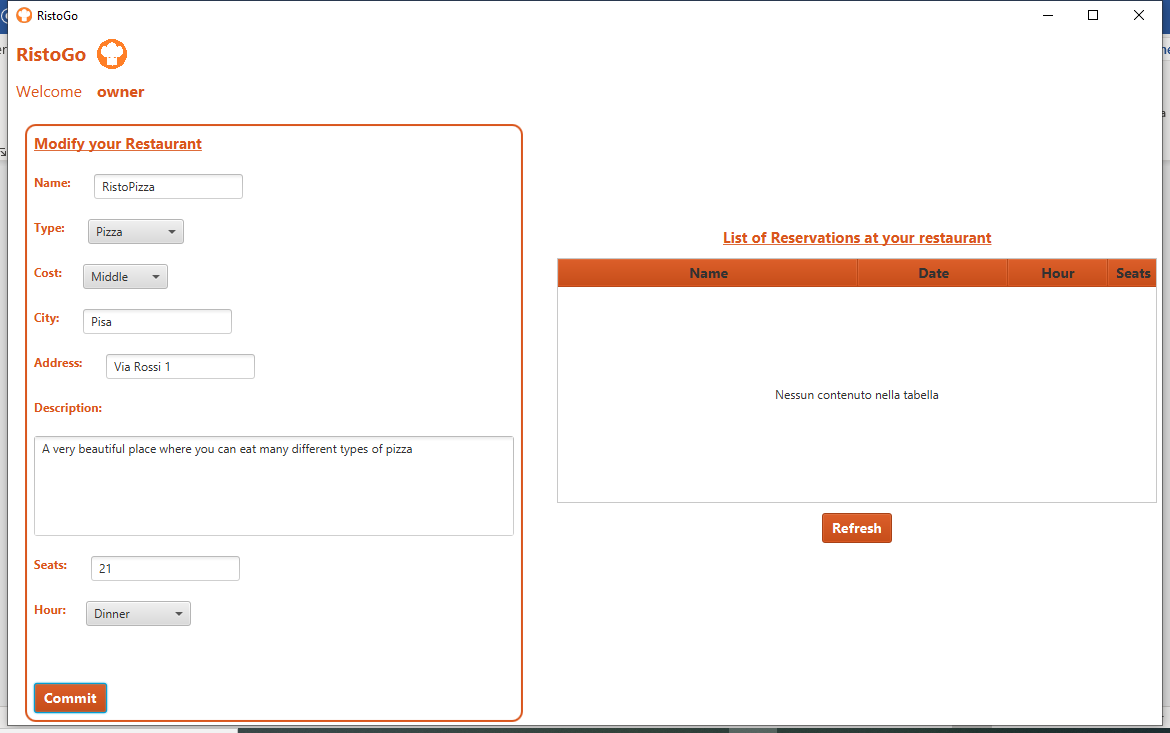
\includegraphics[width=\textwidth]{editrestaurant}
	\caption{Modify restaurant's informations.}
	\label{fig:editrestaurant}
\end{figure}

\subsection{Manage reservations}

In the section ``List of reservations'' you can see all your active
reservations.  The ones of past days are not shown. The list is not updated
automatically. To see the changes, you have to click on button ``Refresh''
(Figure~\ref{fig:managereservations}).

\begin{figure}[!ht]
	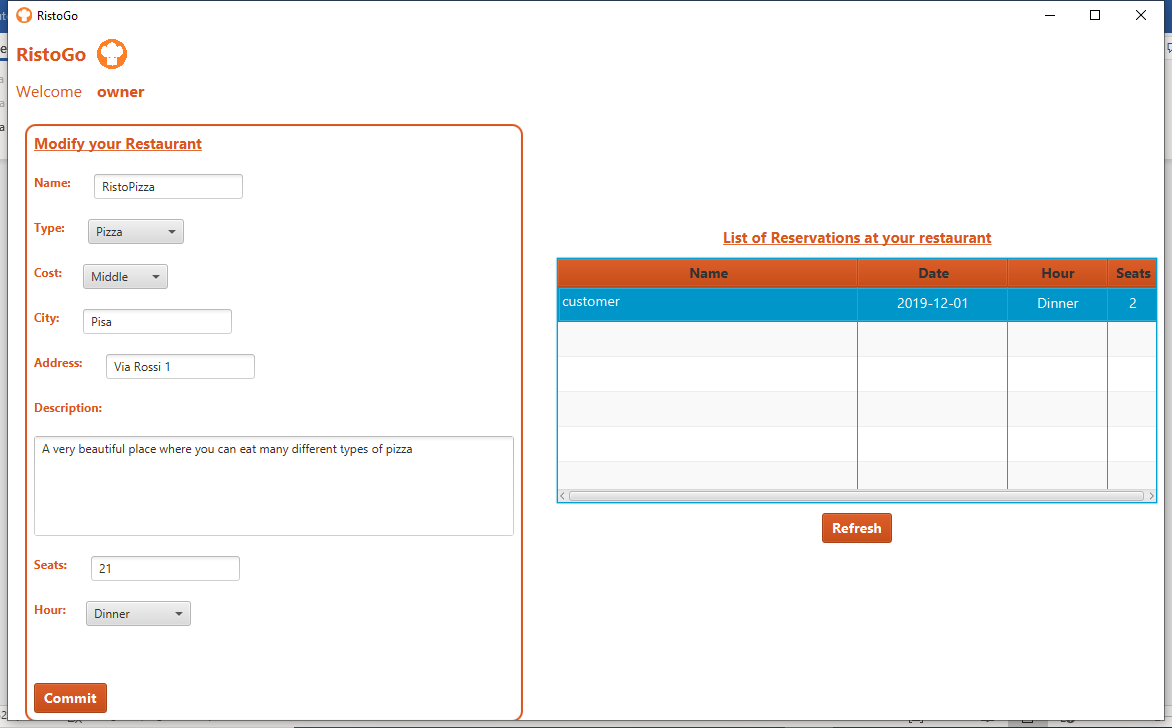
\includegraphics[width=\textwidth]{managereservations}
	\caption{Reservation list.}
	\label{fig:managereservations}
\end{figure}
